\section{Tutoriel}
Le tutoriel du projet se présente sous la forme d'une application \textbf{Linux} développée en \textbf{Python} permettant d'exploiter les quatre types d'attaques présentées précédemment. Disponible à l'adresse suivante: \url{https://github.com/ferreolpennel/Krokmou}, cette application de démonstration est utilisable par tout utilisateur satisfaisant les pré-requis à son installation. L'application, appelée \bsc{Krokmou}, est dédiée à l'ARDrone 2.0 et ne permet des attaques que contre ce type de drone et ce à des fins de démonstration uniquement. Elle permet ainsi de prendre le contrôle d'un drone à la place d'un utilisateur légitime déjà connecté au drone, d'envoyer des commandes pirates au drone sans déconnecter l'utilisateur légitime de celui-ci et de déposer un virus de démonstration sur le drone. Elle illustre ainsi les attaques présentées précédemment et met en relief les failles correspondantes sur ce type de drone.

\subsection{Initialisation de l'application}
L'application permet de sélectionner l'interface Wifi à utiliser pour se connecter au drone. Elle réalise ensuite un scan des réseaux Wifi alentours et affiche ensuite uniquement les réseaux Wifi de drones \textbf{Parrot}. Il suffit à l'attaquant de sélectionner le drone auquel il veut se connecter puis l'application configure l'interface Wifi pour se connecter à celui-ci.

\begin{figure}[H]
  \centering
  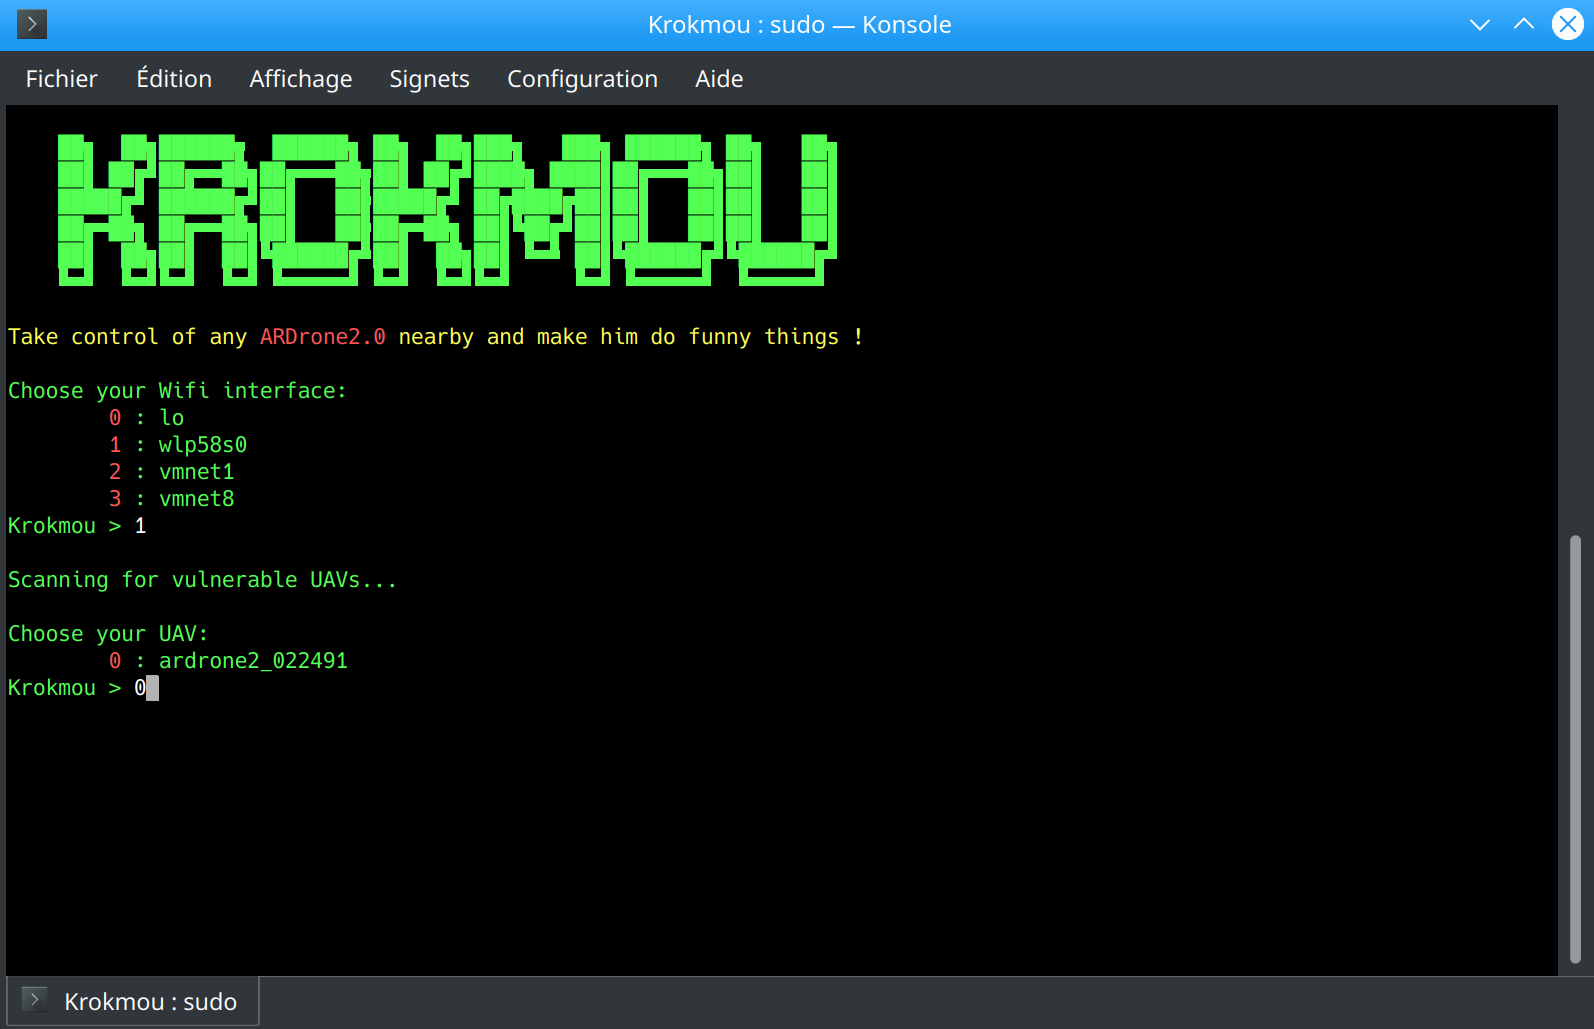
\includegraphics[scale=0.35]{images/opening.png}
  \caption{Initialisation de l'application}
\end{figure}

\subsection{Menu principal}
Le menu principal de l'application permet de sélectionner une des quatre attaques afin de la réaliser sur le drone auquel l'attaquant s'est connecté précédemment.

\begin{figure}[H]
  \centering
  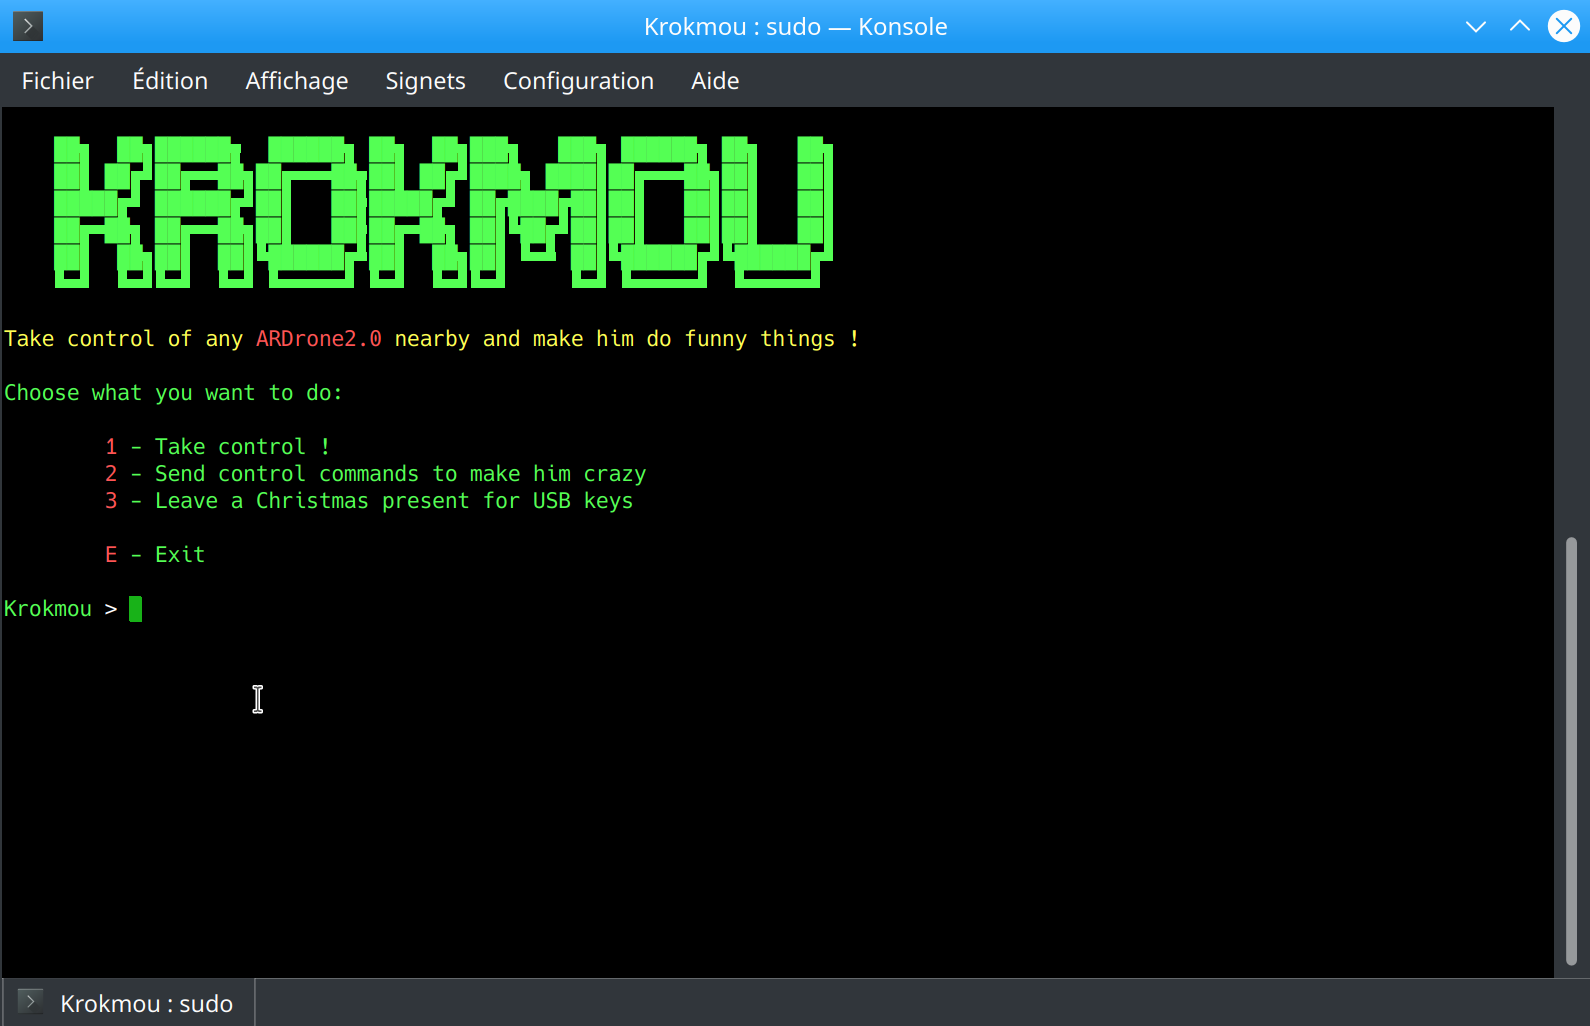
\includegraphics[scale=0.5]{images/main_menu}
  \caption{Menu principal de l'application}
\end{figure}

\subsection{Prise de contrôle du drone}
Cette option du menu permet à l'attaquant de prendre le contrôle du drone à la place de l'utilisateur légitime grâce à l'attaque décrite précédemment dans ce rapport. Le contrôle du drone se réalise au travers du navigateur Web et d'un serveur \textbf{Node.js} issu du dépôt Github suivant: (\url{https://github.com/functino/drone-browser}).\cite{ref5}

\begin{figure}[H]
  \centering
  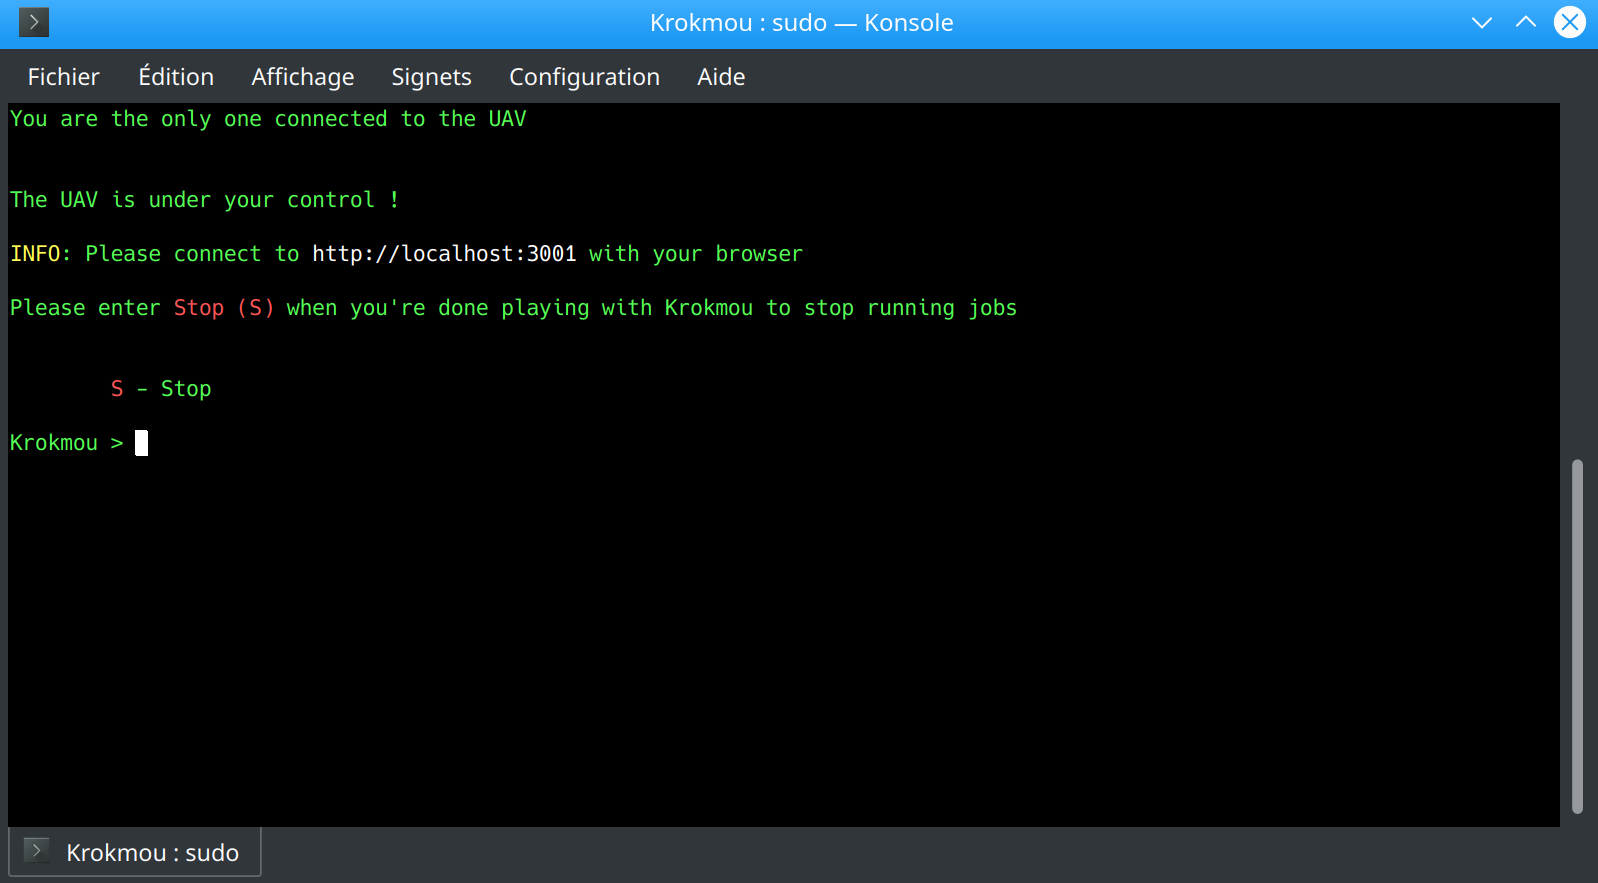
\includegraphics[scale=0.35]{images/taking_control.png}
  \caption{Prise de contrôle du drone par l'application}
\end{figure}

\begin{figure}[H]
  \centering
  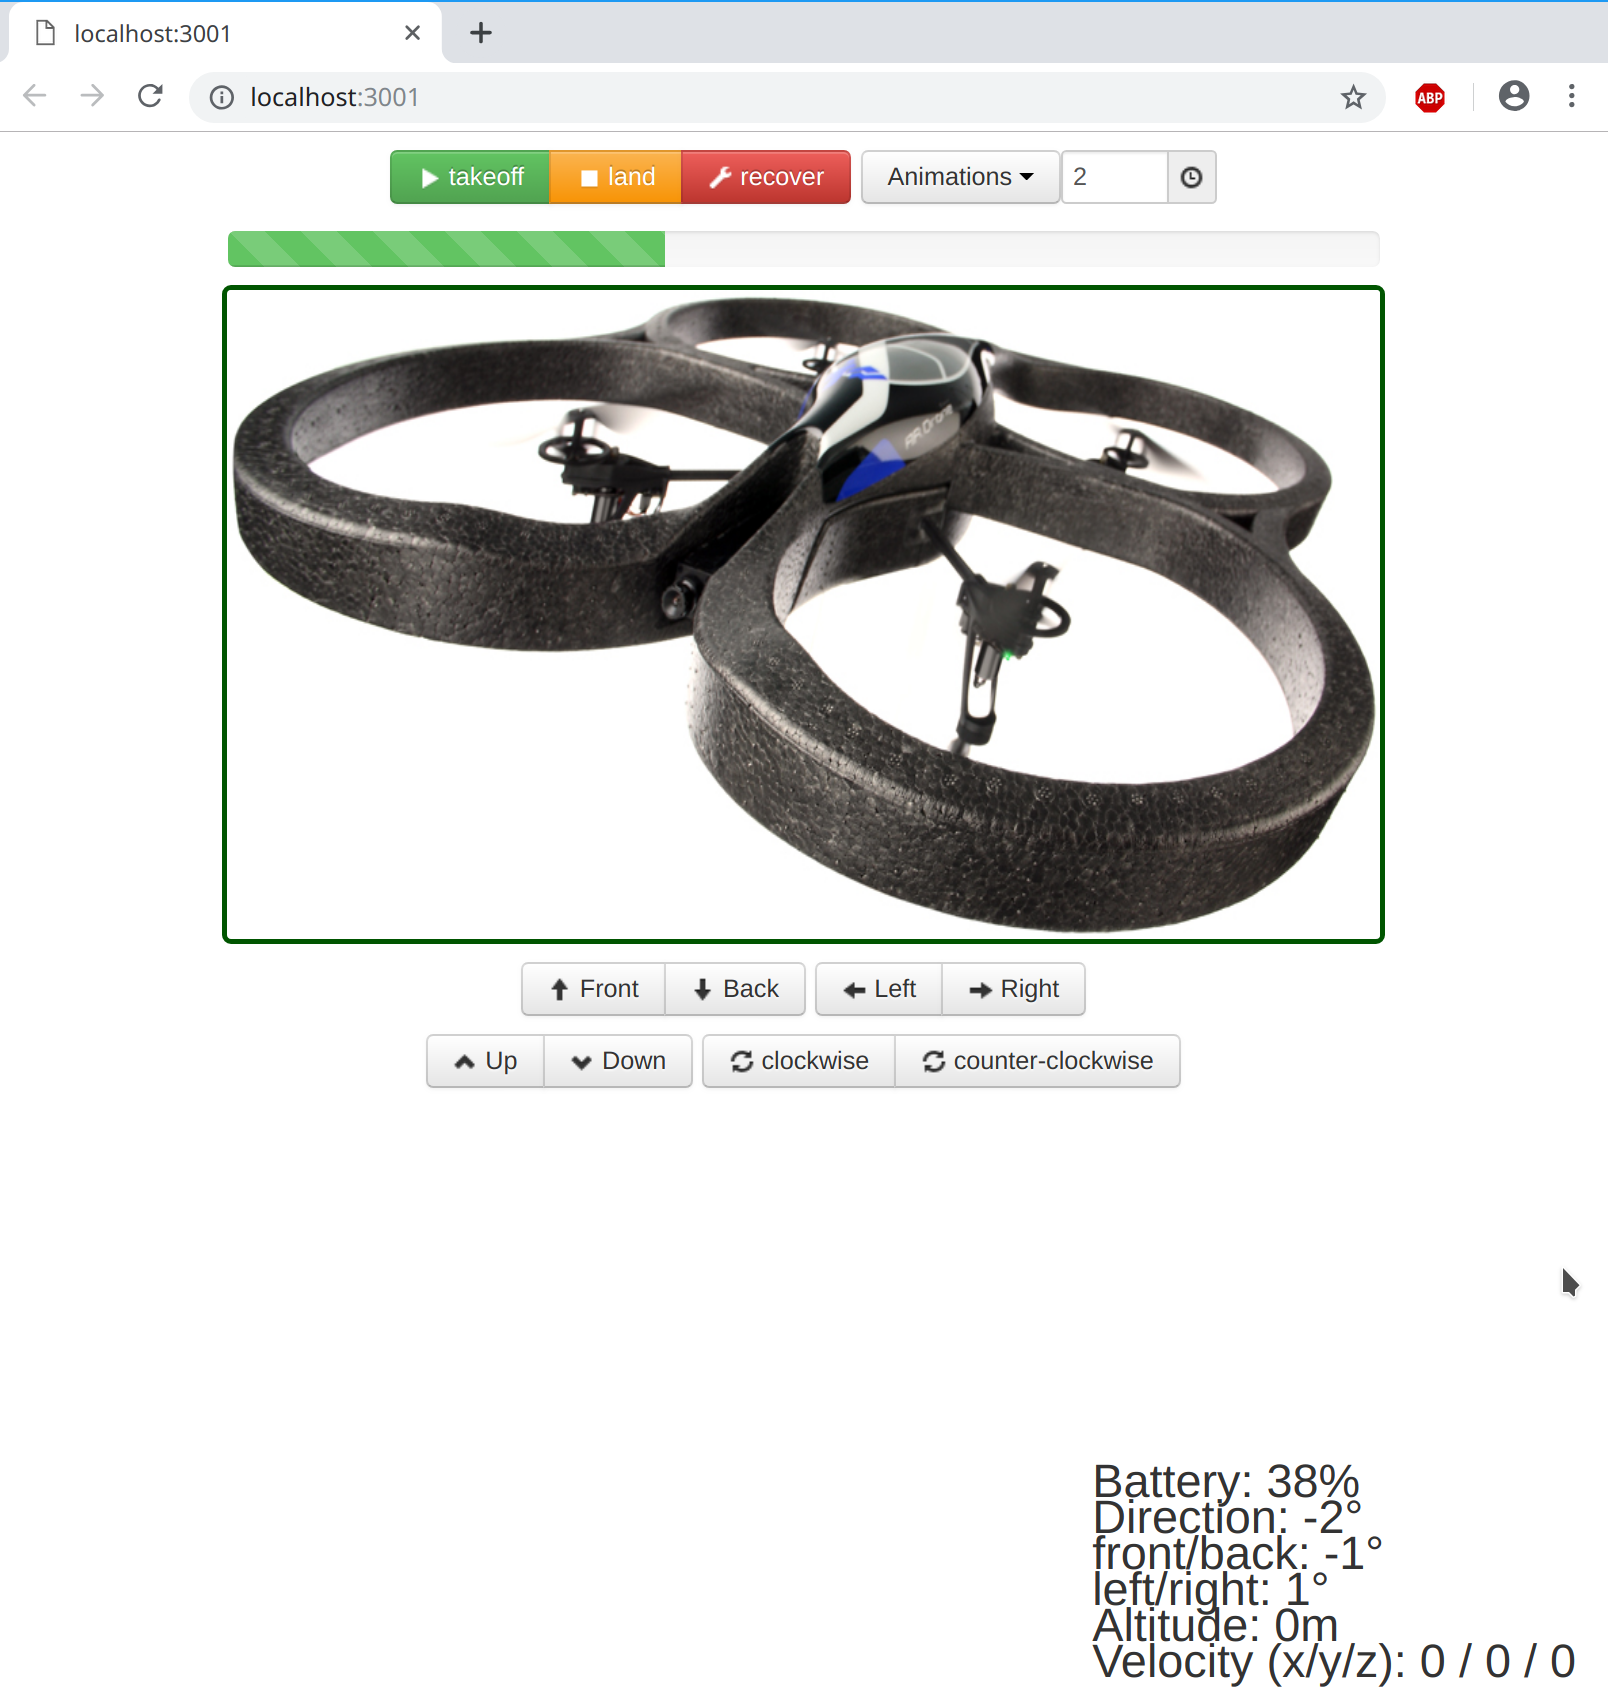
\includegraphics[scale=0.35]{images/control_application.png}
  \caption{Interface de contrôle web}
\end{figure}

\subsection{Injection de commandes}
Ce sous-menu permet à l'attaquant d'envoyer des commandes au drone en laissant le contrôle du drone au client légitime. Les différentes injections de commandes possibles sont présentées dans l'affichage du contrôleur pour l'injection de commandes.

\begin{figure}[H]
  \centering
  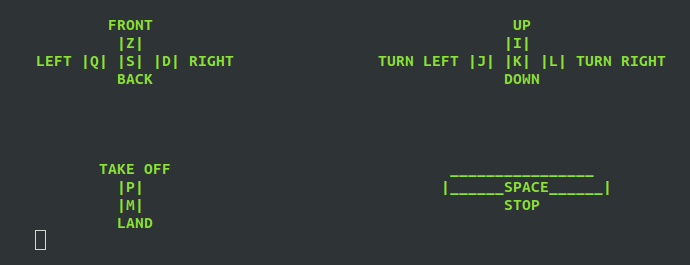
\includegraphics[scale=0.6]{images/injection_command_controler.png}
  \caption{Sous-menu d'injection de commandes}
\end{figure}

Il est donc possible de faire avancer/reculer, d'aller à gauche/droite, de monter/descendre, de tourner à gauche/droite selon l'axe vertical et de décoller/atterrir. L'utilisation du contrôleur se fait donc à l'aide du clavier. \\
Le client légitime garde le contrôle du drone à la seule condition que le drone soit dans le même état (en vol/au sol) que celui du client légitime avant l'injection de commandes.

\subsection{Dépose de virus sur le drone}
Cette option permet d'exploiter une vulnérabilité laissant à l'attaquant un contrôle total du drone. Dans le cadre de la démonstration, l'application dépose un virus et un fichier sélectionné par l'utilisateur sur le drone. Ce fichier sera copié sur toute clé USB qui sera connectée au drone. Celle-ci sera par conséquent considérée comme infectée. Par défaut, l'application dépose le virus et une image sur le drone. C'est cette image qui sera copiée sur toute clé USB connectée au drone toujours à des fins de démonstration. Cependant, l'attaquant peut indiquer le chemin d'un fichier de son choix au moment où l'application lui propose afin de remplacer cette image.

\begin{figure}[H]
  \centering
  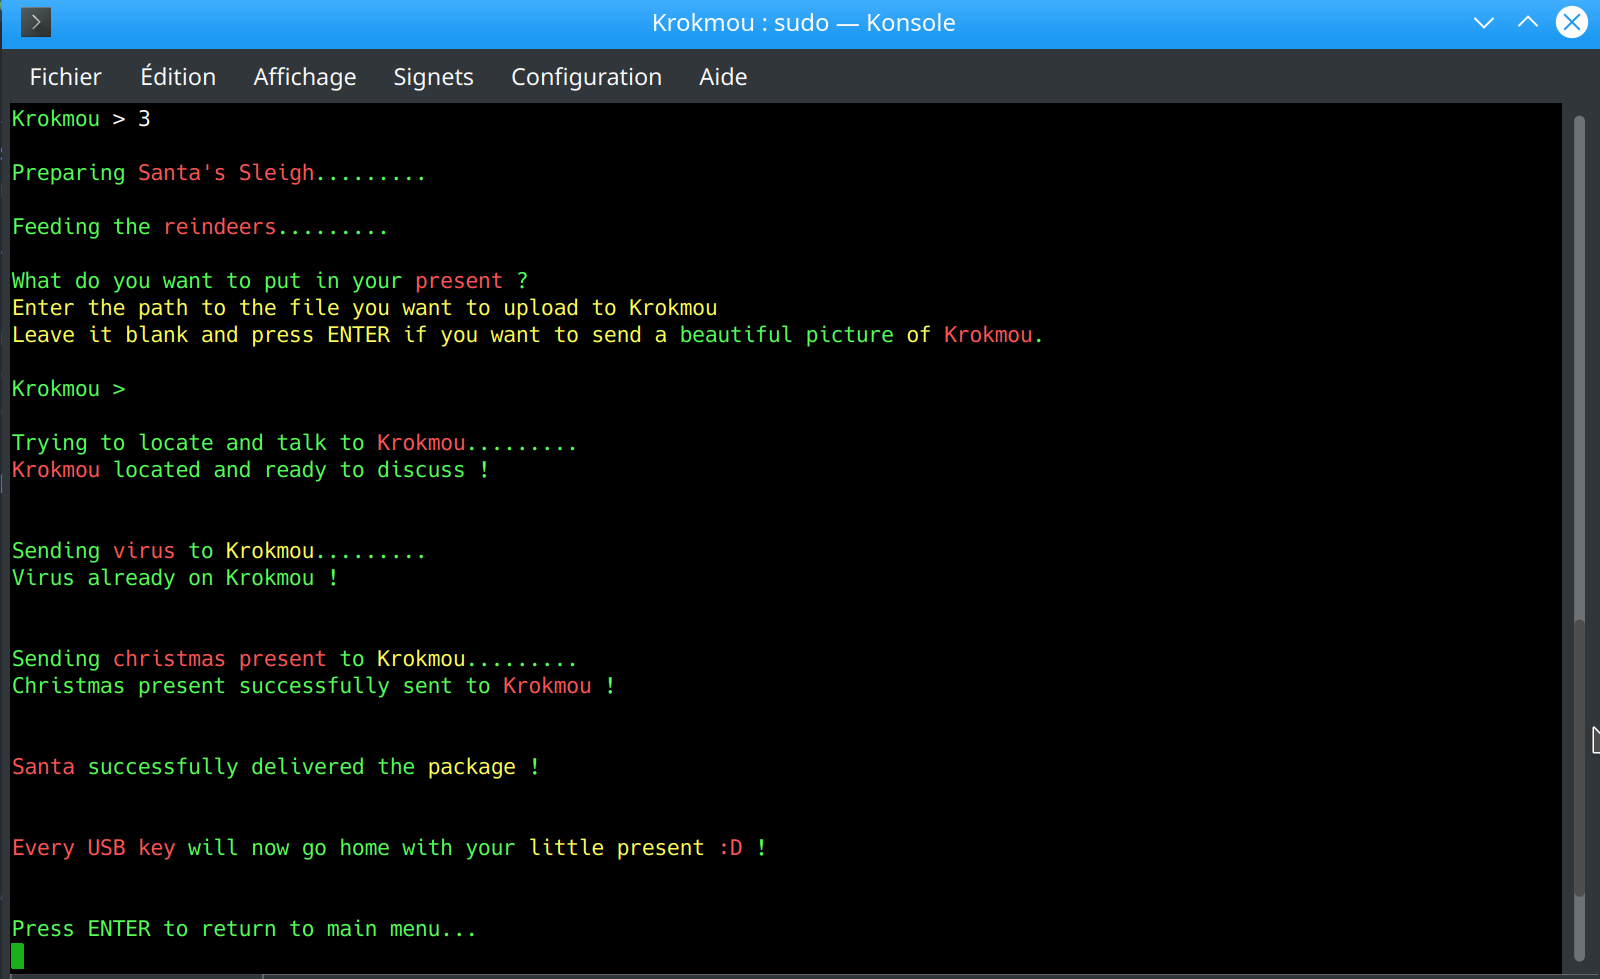
\includegraphics[scale=0.3]{images/virus.png}
  \caption{Envoi du virus et du fichier sur le drone}
\end{figure}

\subsection{Déni de service}
La dernière option permet de réaliser l'attaque de "l'Homme du milieu" sur le client. Une fois selectionnées, cette option permet de bloquer le lien entre le client et le drone. Onpeut au choix bloquer toute les communications avec le drone ou alors bloquer seulement la liason de commande et laisser la liaison vidéo au client.

\begin{figure}[H]
  \centering
  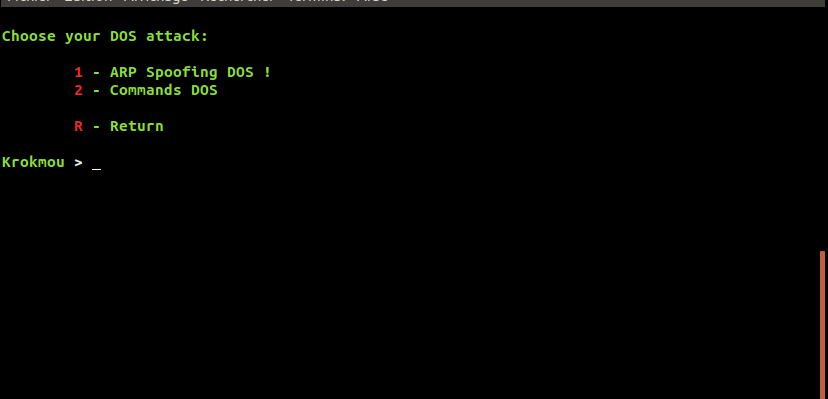
\includegraphics[scale=0.5]{images/dos}
  \caption{Déni de service sur le drone}
\end{figure}
